% libraries:
% Text symbols LaTeX takes from the TS1 encoding (D87): \$ in the roman, bold, italic, sans and typewriter families and several sizes, and a few other textcomp symbols.
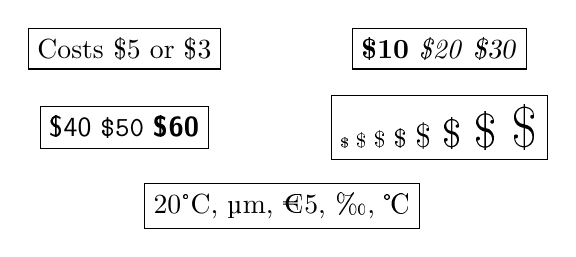
\begin{tikzpicture}
  \node[draw] (a) at (0,0) {Costs \$5 or \textdollar 3};
  \node[draw] (b) at (4,0) {\textbf{\$10} \textit{\$20} \textsl{\$30}};
  \node[draw] (c) at (0,-1) {\textsf{\$40} \texttt{\$50} \textsf{\bfseries\$60}};
  \node[draw] (d) at (4,-1) {\tiny\$ \scriptsize\$ \footnotesize\$ \small\$ \large\$ \Large\$ \LARGE\$ \huge\$};
  \node[draw] (e) at (2,-2) {20\textdegree C, \textmu m, \texteuro 5, \textperthousand, \textcelsius};
\end{tikzpicture}
